%% triangle3.tex
\documentclass{standalone}
\usepackage{tkz-euclide}
\usetkzobj{all}
%% ================== commands ==========================
\newcommand{\myShowPoints}[2]{
\tkzDrawPoints(#1) 
\tkzLabelPoints[#2](#1)
}		
\newcommand{\myProjection}[4]{
% \tkzDefLine[orthogonal=through #1](#3,#2)
% \tkzInterLL(#2,#3)(#1,tkzPointResult) \tkzGetPoint{#4}
\tkzDefPointBy[projection=onto #2--#3](#1) \tkzGetPoint{#4}
\tkzDrawSegments(#1,#4)
\tkzMarkRightAngle[fill=gray!10, scale=.7](#1,#4,#2)
	
}



\begin{document}
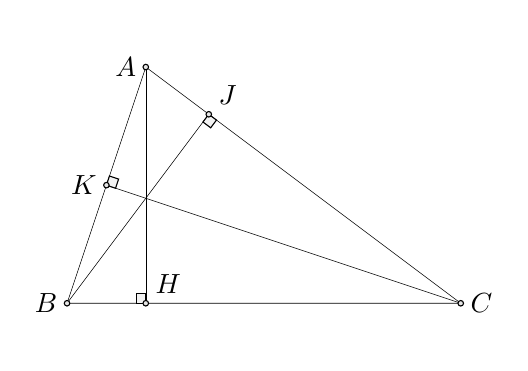
\begin{tikzpicture}
	\clip (-.5,-.5) rectangle (5.5, 3.5);
	\tkzDefPoints{1/3/A, 0/0/B, 5/0/C}
	\tkzDrawPolygon(A,B,C)

	\myProjection{A}{B}{C}{H}
	\myProjection{B}{C}{A}{J}
	\myProjection{C}{A}{B}{K}

	\myShowPoints{A,B}{left}
	\myShowPoints{C}{right}
	\myShowPoints{H, J}{above right}
	\myShowPoints{K}{left}
\end{tikzpicture}
\end{document}